
%(BEGIN_QUESTION)
% Copyright 2015, Tony R. Kuphaldt, released under the Creative Commons Attribution License (v 1.0)
% This means you may do almost anything with this work of mine, so long as you give me proper credit

This loop sheet shows a pneumatic reactor temperature control system utilizing a solenoid valve to assist in the actuation of process valve TV-135:

$$\includegraphics[width=15.5cm]{i0016rx01.eps}$$

Determine the following, based on a close inspection and analysis of the diagram:

\begin{itemize}
\item{} The typical status of the output switch contact on TY-135 ({\it NO} or {\it NC})
\vskip 10pt
\item{} The effect of an AC power loss from breaker \#4
\vskip 10pt
\item{} The effect of the solenoid vent becoming plugged or accidently capped by a technician
\end{itemize}

\underbar{file i00952}
%(END_QUESTION)





%(BEGIN_ANSWER)

\begin{itemize}
\item{} The typical status of the output switch contact on TY-135 ({\it NO} or {\it NC}) -- {\it TY-135's output must typically be conducting (switch contacts closed) in order to pass AC power on to the coil of the solenoid valve and maintain its ``normally energized'' status.}
\vskip 10pt
\item{} The effect of an AC power loss from breaker \#4 -- {\it the solenoid coil would de-energized, venting air pressure from the input of TV-135 and causing that process valve to go to its ``fail'' (closed) position.}
\vskip 10pt
\item{} The effect of the solenoid vent becoming plugged or accidently capped by a technician -- {\it If ever the discrete controller TY-135 commands the solenoid valve to trip, it would force TV-135 to hold its position rather than close as it should.}
\end{itemize}

%(END_ANSWER)





%(BEGIN_NOTES)


%INDEX% Documentation, loop diagram: realistic industrial example 
%INDEX% Final Control Elements, valve: fail-safe solenoids

%(END_NOTES)


